\documentclass{standalone}
\usepackage{tikz}
\usetikzlibrary{patterns, positioning}
\usepackage[sfdefault]{ClearSans} %% option 'sfdefault' activates Clear Sans as the default text font
\usepackage[T1]{fontenc}

\begin{document}
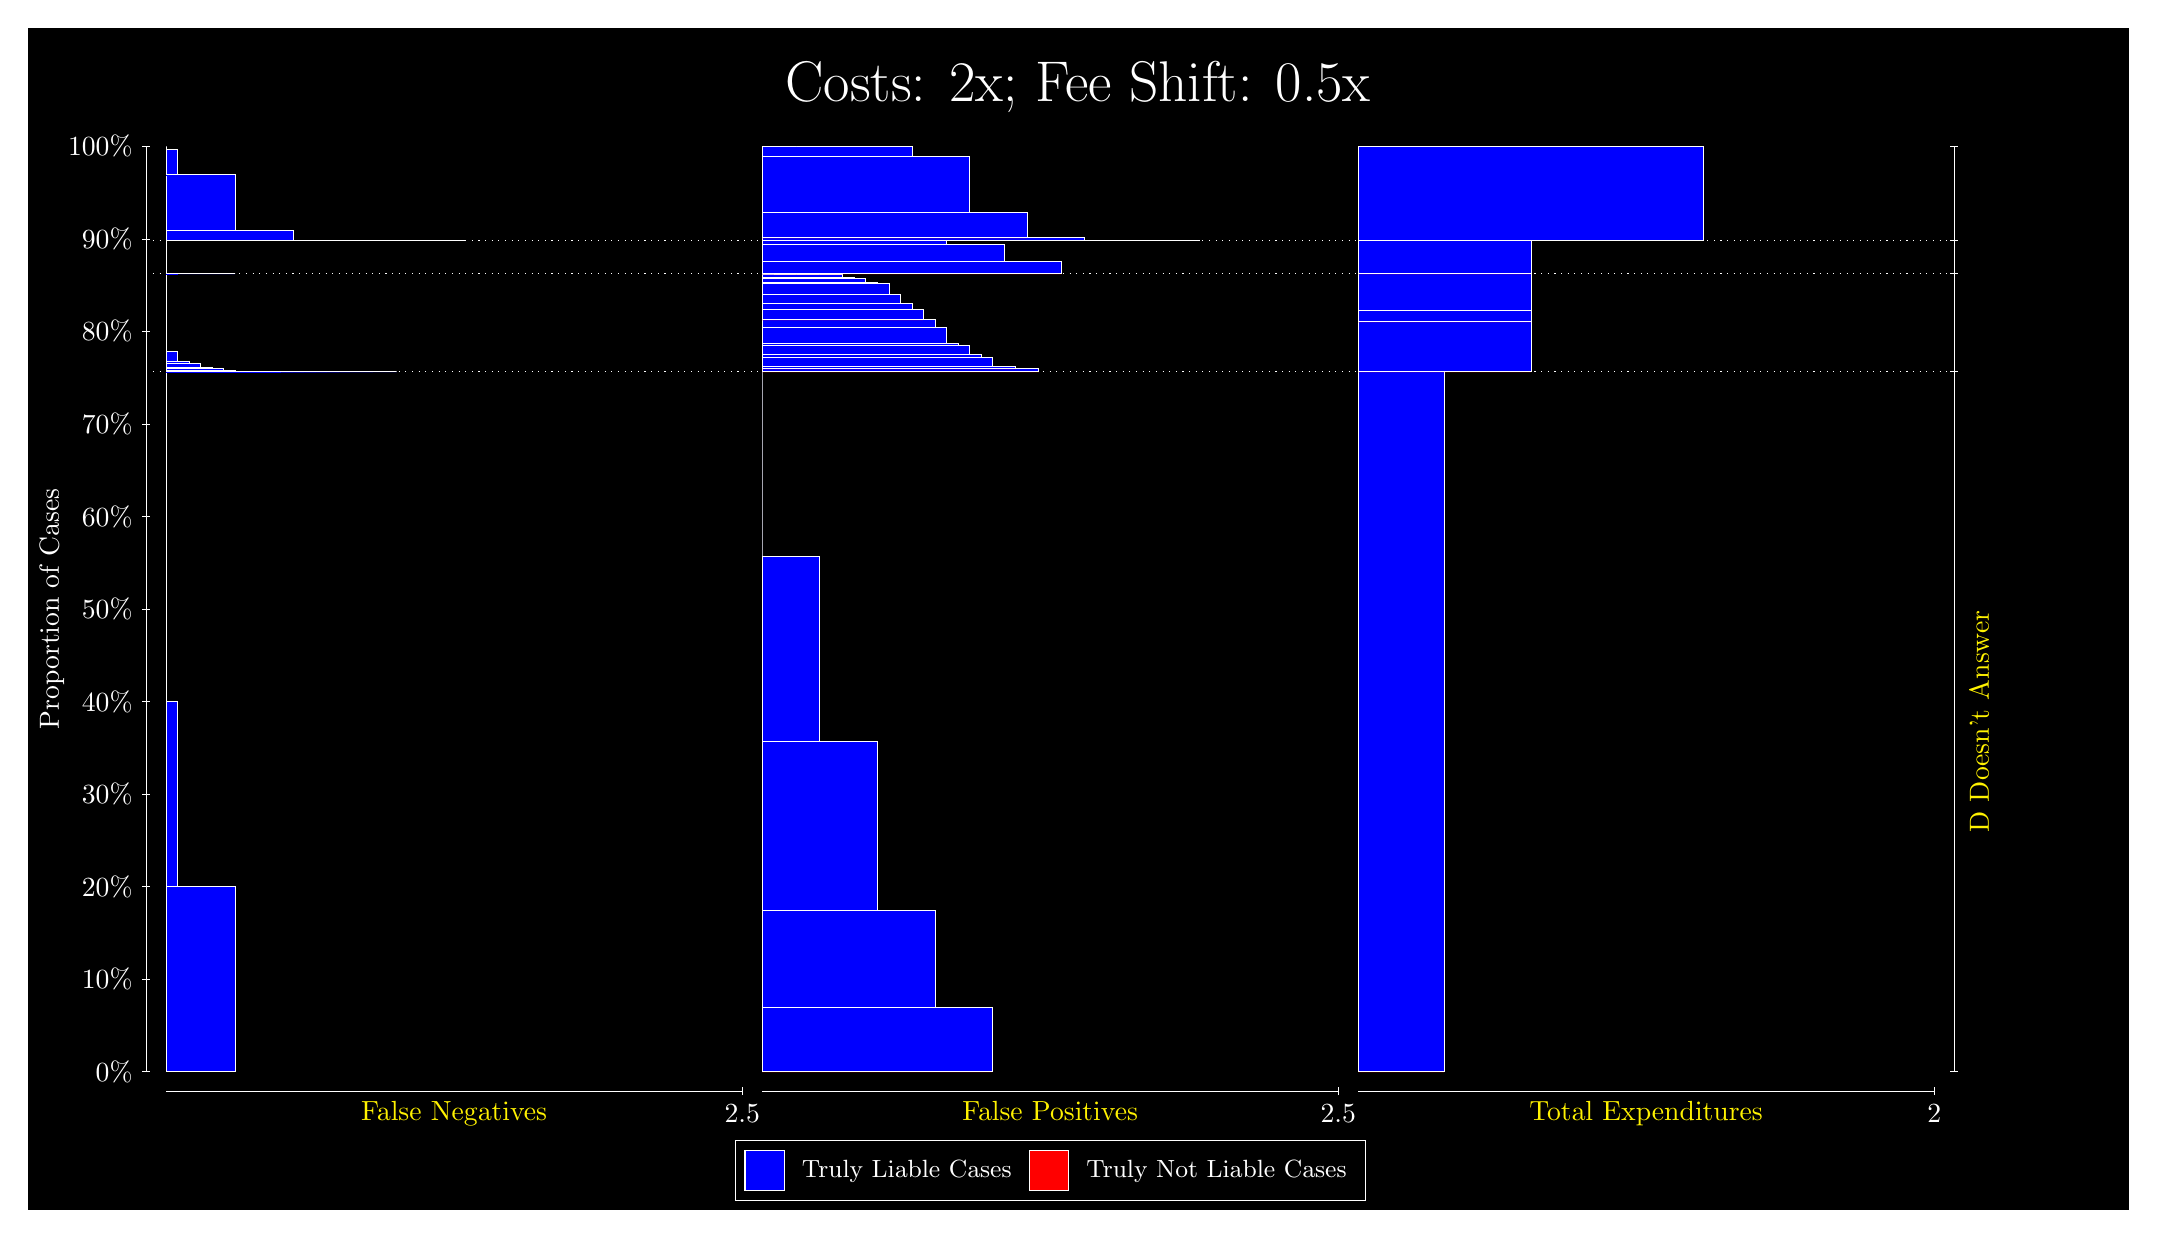
\begin{tikzpicture}
\draw[fill=black] (0,0) rectangle (26.667,15);
\draw[text=white] (0,13.5) rectangle (26.667,15) node[midway] {\huge Costs: 2x; Fee Shift: 0.5x};
\draw[white, very thin] (1.5,1.75) -- (1.5,13.5);
\node[rotate=90, text=white, anchor=center] at (0.3, 7.625) {Proportion of Cases};
\draw[white, very thin] (1.45,1.75) -- (1.55,1.75);
\node[text=white, anchor=east] at (1.45, 1.75) {0\%};
\draw[white, very thin] (1.45,2.925) -- (1.55,2.925);
\node[text=white, anchor=east] at (1.45, 2.925) {10\%};
\draw[white, very thin] (1.45,4.1) -- (1.55,4.1);
\node[text=white, anchor=east] at (1.45, 4.1) {20\%};
\draw[white, very thin] (1.45,5.275) -- (1.55,5.275);
\node[text=white, anchor=east] at (1.45, 5.275) {30\%};
\draw[white, very thin] (1.45,6.45) -- (1.55,6.45);
\node[text=white, anchor=east] at (1.45, 6.45) {40\%};
\draw[white, very thin] (1.45,7.625) -- (1.55,7.625);
\node[text=white, anchor=east] at (1.45, 7.625) {50\%};
\draw[white, very thin] (1.45,8.8) -- (1.55,8.8);
\node[text=white, anchor=east] at (1.45, 8.8) {60\%};
\draw[white, very thin] (1.45,9.975) -- (1.55,9.975);
\node[text=white, anchor=east] at (1.45, 9.975) {70\%};
\draw[white, very thin] (1.45,11.15) -- (1.55,11.15);
\node[text=white, anchor=east] at (1.45, 11.15) {80\%};
\draw[white, very thin] (1.45,12.325) -- (1.55,12.325);
\node[text=white, anchor=east] at (1.45, 12.325) {90\%};
\draw[white, very thin] (1.45,13.5) -- (1.55,13.5);
\node[text=white, anchor=east] at (1.45, 13.5) {100\%};

\draw[white, very thin] (24.457,1.75) -- (24.457,13.5);
\draw[white, very thin] (24.407,1.75) -- (24.507,1.75);
\node[anchor=west] at (24.407, 1.75) {};
\draw[white, very thin] (24.407,10.638) -- (24.507,10.638);
\node[anchor=west] at (24.407, 10.638) {};
\draw[white, very thin] (24.407,11.882) -- (24.507,11.882);
\node[anchor=west] at (24.407, 11.882) {};
\draw[white, very thin] (24.407,12.309) -- (24.507,12.309);
\node[anchor=west] at (24.407, 12.309) {};
\draw[white, very thin] (24.407,13.5) -- (24.507,13.5);
\node[anchor=west] at (24.407, 13.5) {};

\draw[white, very thin, fill=blue] (1.75,1.75) rectangle (2.6283,4.0999);
\draw[white, very thin, fill=blue] (1.75,4.0999) rectangle (1.8964,6.4482);
\draw[white, very thin, fill=red] (1.75,6.4482) rectangle (1.75,6.4482);
\draw[white, very thin, fill=blue] (1.75,6.4482) rectangle (1.75,10.638);
\draw[white, very thin, fill=blue] (1.75,10.638) rectangle (4.6775,10.638);
\draw[white, very thin, fill=blue] (1.75,10.638) rectangle (4.3848,10.638);
\draw[white, very thin, fill=blue] (1.75,10.638) rectangle (4.092,10.638);
\draw[white, very thin, fill=blue] (1.75,10.638) rectangle (3.9457,10.638);
\draw[white, very thin, fill=blue] (1.75,10.638) rectangle (3.7993,10.638);
\draw[white, very thin, fill=blue] (1.75,10.638) rectangle (3.6529,10.638);
\draw[white, very thin, fill=blue] (1.75,10.638) rectangle (3.5065,10.638);
\draw[white, very thin, fill=blue] (1.75,10.638) rectangle (3.3602,10.638);
\draw[white, very thin, fill=blue] (1.75,10.638) rectangle (3.2138,10.639);
\draw[white, very thin, fill=blue] (1.75,10.639) rectangle (3.0674,10.639);
\draw[white, very thin, fill=blue] (1.75,10.639) rectangle (2.921,10.641);
\draw[white, very thin, fill=blue] (1.75,10.641) rectangle (2.921,10.641);
\draw[white, very thin, fill=blue] (1.75,10.641) rectangle (2.7746,10.641);
\draw[white, very thin, fill=blue] (1.75,10.641) rectangle (2.6283,10.65);
\draw[white, very thin, fill=blue] (1.75,10.65) rectangle (2.4819,10.685);
\draw[white, very thin, fill=blue] (1.75,10.685) rectangle (2.3355,10.691);
\draw[white, very thin, fill=blue] (1.75,10.691) rectangle (2.1891,10.747);
\draw[white, very thin, fill=blue] (1.75,10.747) rectangle (2.1891,10.747);
\draw[white, very thin, fill=blue] (1.75,10.747) rectangle (2.0428,10.765);
\draw[white, very thin, fill=blue] (1.75,10.765) rectangle (1.8964,10.898);
\draw[white, very thin, fill=red] (1.75,10.898) rectangle (1.75,10.898);
\draw[white, very thin, fill=blue] (1.75,10.898) rectangle (1.75,11.882);
\draw[white, very thin, fill=blue] (1.75,11.882) rectangle (2.6283,11.882);
\draw[white, very thin, fill=blue] (1.75,11.882) rectangle (1.8964,11.883);
\draw[white, very thin, fill=red] (1.75,11.883) rectangle (1.75,11.883);
\draw[white, very thin, fill=blue] (1.75,11.883) rectangle (1.75,12.309);
\draw[white, very thin, fill=blue] (1.75,12.309) rectangle (5.5558,12.309);
\draw[white, very thin, fill=blue] (1.75,12.309) rectangle (4.8239,12.309);
\draw[white, very thin, fill=blue] (1.75,12.309) rectangle (4.092,12.311);
\draw[white, very thin, fill=blue] (1.75,12.311) rectangle (3.3602,12.438);
\draw[white, very thin, fill=blue] (1.75,12.438) rectangle (2.6283,12.438);
\draw[white, very thin, fill=blue] (1.75,12.438) rectangle (2.6283,13.141);
\draw[white, very thin, fill=blue] (1.75,13.141) rectangle (1.8964,13.142);
\draw[white, very thin, fill=blue] (1.75,13.142) rectangle (1.8964,13.468);
\draw[white, very thin, fill=red] (1.75,13.468) rectangle (1.75,13.468);
\draw[white, very thin, fill=blue] (1.75,13.468) rectangle (1.75,13.5);
\draw[white, very thin, fill=red] (9.3189,1.75) rectangle (12.246,1.75);
\draw[white, very thin, fill=blue] (9.3189,1.75) rectangle (12.246,2.5688);
\draw[white, very thin, fill=blue] (9.3189,2.5688) rectangle (11.515,3.7934);
\draw[white, very thin, fill=blue] (9.3189,3.7934) rectangle (10.783,5.94);
\draw[white, very thin, fill=blue] (9.3189,5.94) rectangle (10.051,8.2883);
\draw[white, very thin, fill=blue] (9.3189,8.2883) rectangle (9.3189,10.638);
\draw[white, very thin, fill=red] (9.3189,10.638) rectangle (12.832,10.638);
\draw[white, very thin, fill=blue] (9.3189,10.638) rectangle (12.832,10.677);
\draw[white, very thin, fill=red] (9.3189,10.677) rectangle (12.539,10.677);
\draw[white, very thin, fill=blue] (9.3189,10.677) rectangle (12.539,10.711);
\draw[white, very thin, fill=red] (9.3189,10.711) rectangle (12.246,10.711);
\draw[white, very thin, fill=blue] (9.3189,10.711) rectangle (12.246,10.819);
\draw[white, very thin, fill=blue] (9.3189,10.819) rectangle (12.1,10.858);
\draw[white, very thin, fill=red] (9.3189,10.858) rectangle (11.954,10.858);
\draw[white, very thin, fill=blue] (9.3189,10.858) rectangle (11.954,10.973);
\draw[white, very thin, fill=blue] (9.3189,10.973) rectangle (11.807,11.005);
\draw[white, very thin, fill=red] (9.3189,11.005) rectangle (11.661,11.005);
\draw[white, very thin, fill=blue] (9.3189,11.005) rectangle (11.661,11.202);
\draw[white, very thin, fill=blue] (9.3189,11.202) rectangle (11.515,11.299);
\draw[white, very thin, fill=red] (9.3189,11.299) rectangle (11.368,11.299);
\draw[white, very thin, fill=blue] (9.3189,11.299) rectangle (11.368,11.425);
\draw[white, very thin, fill=blue] (9.3189,11.425) rectangle (11.222,11.503);
\draw[white, very thin, fill=blue] (9.3189,11.503) rectangle (11.075,11.51);
\draw[white, very thin, fill=red] (9.3189,11.51) rectangle (11.075,11.51);
\draw[white, very thin, fill=blue] (9.3189,11.51) rectangle (11.075,11.623);
\draw[white, very thin, fill=blue] (9.3189,11.623) rectangle (10.929,11.755);
\draw[white, very thin, fill=blue] (9.3189,11.755) rectangle (10.783,11.774);
\draw[white, very thin, fill=blue] (9.3189,11.774) rectangle (10.636,11.83);
\draw[white, very thin, fill=blue] (9.3189,11.83) rectangle (10.49,11.835);
\draw[white, very thin, fill=blue] (9.3189,11.835) rectangle (10.344,11.835);
\draw[white, very thin, fill=blue] (9.3189,11.835) rectangle (10.344,11.87);
\draw[white, very thin, fill=blue] (9.3189,11.87) rectangle (10.197,11.88);
\draw[white, very thin, fill=blue] (9.3189,11.88) rectangle (10.051,11.88);
\draw[white, very thin, fill=blue] (9.3189,11.88) rectangle (9.9044,11.881);
\draw[white, very thin, fill=blue] (9.3189,11.881) rectangle (9.758,11.881);
\draw[white, very thin, fill=blue] (9.3189,11.881) rectangle (9.6116,11.881);
\draw[white, very thin, fill=blue] (9.3189,11.881) rectangle (9.6116,11.882);
\draw[white, very thin, fill=blue] (9.3189,11.882) rectangle (9.4652,11.882);
\draw[white, very thin, fill=blue] (9.3189,11.882) rectangle (9.3189,11.882);
\draw[white, very thin, fill=red] (9.3189,11.882) rectangle (13.125,11.882);
\draw[white, very thin, fill=blue] (9.3189,11.882) rectangle (13.125,12.043);
\draw[white, very thin, fill=blue] (9.3189,12.043) rectangle (12.393,12.253);
\draw[white, very thin, fill=blue] (9.3189,12.253) rectangle (11.661,12.308);
\draw[white, very thin, fill=blue] (9.3189,12.308) rectangle (10.929,12.309);
\draw[white, very thin, fill=blue] (9.3189,12.309) rectangle (10.197,12.309);
\draw[white, very thin, fill=red] (9.3189,12.309) rectangle (14.881,12.309);
\draw[white, very thin, fill=blue] (9.3189,12.309) rectangle (14.881,12.309);
\draw[white, very thin, fill=red] (9.3189,12.309) rectangle (14.149,12.309);
\draw[white, very thin, fill=blue] (9.3189,12.309) rectangle (14.149,12.309);
\draw[white, very thin, fill=red] (9.3189,12.309) rectangle (13.417,12.309);
\draw[white, very thin, fill=blue] (9.3189,12.309) rectangle (13.417,12.341);
\draw[white, very thin, fill=red] (9.3189,12.341) rectangle (12.686,12.341);
\draw[white, very thin, fill=blue] (9.3189,12.341) rectangle (12.686,12.667);
\draw[white, very thin, fill=red] (9.3189,12.667) rectangle (11.954,12.667);
\draw[white, very thin, fill=blue] (9.3189,12.667) rectangle (11.954,13.371);
\draw[white, very thin, fill=blue] (9.3189,13.371) rectangle (11.222,13.498);
\draw[white, very thin, fill=blue] (9.3189,13.498) rectangle (10.49,13.5);
\draw[white, very thin, fill=blue] (9.3189,13.5) rectangle (9.758,13.5);
\draw[white, very thin, fill=blue] (9.3189,13.5) rectangle (9.3189,13.5);
\draw[white, very thin, fill=red] (16.888,1.75) rectangle (17.986,1.75);
\draw[white, very thin, fill=blue] (16.888,1.75) rectangle (17.986,10.638);
\draw[white, very thin, fill=red] (16.888,10.638) rectangle (19.083,10.638);
\draw[white, very thin, fill=blue] (16.888,10.638) rectangle (19.083,11.274);
\draw[white, very thin, fill=red] (16.888,11.274) rectangle (19.083,11.274);
\draw[white, very thin, fill=blue] (16.888,11.274) rectangle (19.083,11.422);
\draw[white, very thin, fill=red] (16.888,11.422) rectangle (19.083,11.422);
\draw[white, very thin, fill=blue] (16.888,11.422) rectangle (19.083,11.882);
\draw[white, very thin, fill=red] (16.888,11.882) rectangle (19.083,11.882);
\draw[white, very thin, fill=blue] (16.888,11.882) rectangle (19.083,12.309);
\draw[white, very thin, fill=red] (16.888,12.309) rectangle (21.279,12.309);
\draw[white, very thin, fill=blue] (16.888,12.309) rectangle (21.279,13.5);
\draw[white, dotted] (1.5,10.638) -- (24.457,10.638);
\draw[white, dotted] (1.5,11.882) -- (24.457,11.882);
\draw[white, dotted] (1.5,12.309) -- (24.457,12.309);
\draw[white, very thin] (1.75,1.5) -- (9.0689,1.5);
\node[text=yellow, anchor=north] at (5.4094, 1.5) {False Negatives};
\draw[white, very thin] (9.0689,1.45) -- (9.0689,1.55);
\node[text=white, anchor=north] at (9.0689, 1.45) {2.5};

\draw[white, very thin] (9.3189,1.5) -- (16.638,1.5);
\node[text=yellow, anchor=north] at (12.978, 1.5) {False Positives};
\draw[white, very thin] (16.638,1.45) -- (16.638,1.55);
\node[text=white, anchor=north] at (16.638, 1.45) {2.5};

\draw[white, very thin] (16.888,1.5) -- (24.207,1.5);
\node[text=yellow, anchor=north] at (20.547, 1.5) {Total Expenditures};
\draw[white, very thin] (24.207,1.45) -- (24.207,1.55);
\node[text=white, anchor=north] at (24.207, 1.45) {2};

\node[text=yellow, centered, rotate=90] at (24.777, 6.1941) {D Doesn't Answer};




\draw (12.978300999999998,1.5) node[draw=none] (baseCoordinate) {};
\begin{scope}[align=center]
        \matrix[scale=0.5, draw=white, below=0.5cm of baseCoordinate, nodes={draw}, column sep=0.1cm]{
            \node[rectangle, draw, minimum width=0.5cm, minimum height=0.5cm, fill=blue] {}; &
            \node[draw=none, font=\small, text=white] (B) {Truly Liable Cases}; &
            \node[rectangle, draw, minimum width=0.5cm, minimum height=0.5cm, fill=red] {}; &
            \node[draw=none, font=\small, text=white] (B) {Truly Not Liable Cases}; \\
            };
\end{scope}

\end{tikzpicture}
\end{document}